\subsection{Ethnography Ontology}
This ontology captures the ethnographic details of a location we obtained from the field survey. This data and the ontology can help frame policies and make decisions to mitigate air pollution at the hyperlocal level. The \emph{Ethnography} module is shown in Figure~\ref{fig:ethnographic_concepts}.

\begin{figure}[ht]
\centering
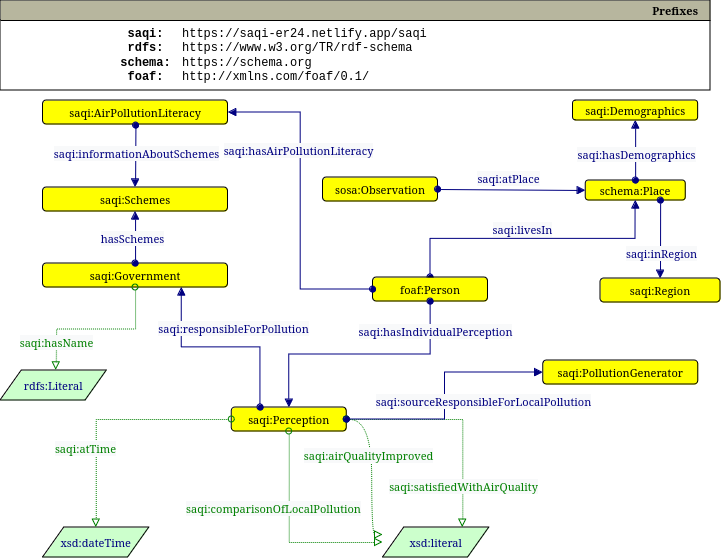
\includegraphics[height=6.5cm]{figures/Ethnography.png}
\caption{Overview of the Ethnography module} 
\label{fig:ethnographic_concepts}
\end{figure}

\textbf{Person.} This is a core concept of this module since the ethnographic data relies on the observations of a person. The data we collect relates a person to their knowledge of air pollution and accounts for the social makeup through the aggregation of person-level data. This concept is connected to concepts such as \texttt{AirPollutionLiteracy}, \texttt{Perception} and \texttt{Region} through the \texttt{hasAirPollution\-Literacy}, \texttt{hasPerception} and \texttt{livesIn} properties.

\textbf{AirPollutionLiteracy.} This concept describes the air pollution literacy of the people in a locality. We assess this by asking questions\footnote{The questionnaire for collecting ethnographic data has been designed by social scientists in our team.} to the people related to their awareness of AQI and air pollution in general. The \texttt{AirPollutionLiteracy} concept has the data properties \texttt{hasAQILiteracy}, \texttt{hasAirPollutionGraphic\-Literacy}, \texttt{hasParticulateMatterLiteracy} and \texttt{hasAQIColorLiteracy}. 

\textbf{Perception.} This concept captures the perception of an individual with regard to the level of air pollution in their local neighbourhood and the city. It consists of data properties such as \texttt{howIsYourLocalityComparedToOtherAreas} (the literals that can be linked using this property are ``equally polluted'', ``less polluted'', ``more polluted'', ``don't know''), \texttt{shouldPollutionIssuesBeRaisedIn\-Elections} and \texttt{localAirQualityRating}. An aggregation of people's perceptions in a particular region is expected to give the perception of that region.

